\documentclass[12pt,twoside]{article}
\usepackage{graphicx}																		
\usepackage[romanian]{babel}
\usepackage[unicode]{hyperref}
\usepackage[dvipsnames]{xcolor} 
\usepackage{amsmath,epsfig,pifont,calc,pifont,pstricks}
\usepackage{rom} 						 % pentru a scrie cu diacritice in limba romana	
\usepackage{color}
\usepackage{listings}
\definecolor{mygreen}{RGB}{28,172,0} % color values Red, Green, Blue
\definecolor{mylilas}{RGB}{170,55,241}
\usepackage{placeins}

\definecolor{ultramarine}{rgb}{0.07, 0.04, 0.56}
\definecolor{Capri}{rgb}{0.0, 0.75, 1.0}
\definecolor{violet}{rgb}{0.56, 0.0, 1.0}

\usepackage{etoolbox}
\patchcmd{\thebibliography}{\chapter*}{\section*}{}{}

%%% setari ale paginii
%indentarea la inceput de paragraf
\setlength{\parindent}{3ex}

%dimensiunea textului pe pagina
\setlength{\voffset}{-2cm}
\setlength{\textheight}{23cm}  
\setlength{\textwidth}{16cm}
\setlength{\topmargin}{0cm}
\setlength{\headsep}{1cm}
\renewcommand{\baselinestretch}{1.2}
\newcommand{\myindent}{\hspace*{3ex}}
%\renewcommand{\baselinestretch}{1}

%margini
\setlength{\oddsidemargin}{0.5cm}
\setlength{\evensidemargin}{-0.3cm}
%\raggedright
\raggedbottom

%% begin preambul - macro-uri definite de autor
\newcommand{\D}{\mathrm{d}}	% va fi folosita in mediul matematic, pentru diferentiala d
\newcommand{\I}{\mathrm{i}}	% va fi folosita in mediul matematic, pentru unitatea imaginara
\newcommand{\eul}{\mathrm{e}}	% numarul lui Euler
\newcommand{\vect}[1]{\mathbf{#1}}	% comanda cu un argument, pentru scrierea vectorilor cu lidere aldine, drepte

\begin{document}
\title{\centering \LARGE{\color{ultramarine}{\textbf{Proiect AD} \\Sound Keyboard\\}}}
\author{Facultatea de Automatic'a 'si Calculatoare\\Universitatea Politehnic'a Bucure'sti\\\\ {\em Du'tu Alin C'alin}}
\maketitle
\newpage
\tableofcontents
\newpage
\section{Introducere}
\myindent
Aceas't'a aplica'tie are numele de Sound Keyboard 'si are rol 'in simularea a 5 sunete de frecven'te diferite utiliz\^and un microcontroller, butoane, difuzor, LED-uri 'si alte componente. Circuitul prezentat are 'si un LCD cu rol 'in afi'sarea mesajelor date de microcontroller.

\vspace{10 mm}
\section{Schema circuitului}

Link: \url{https://www.tinkercad.com/things/dIhJH05zwqa-arduino-circuit}

\vspace{10mm}
\begin{figure}[ht]
\centering
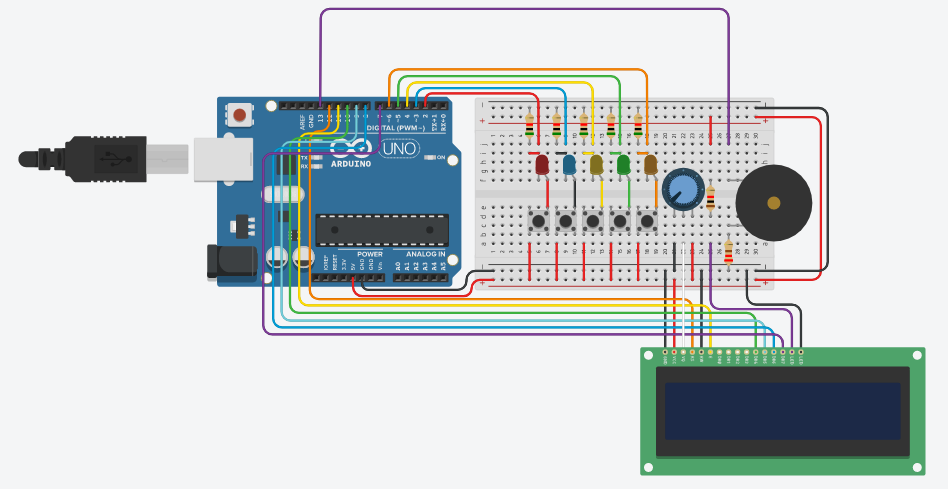
\includegraphics[scale=0.65]{Fisiere/Sound keyboard}
\caption {Schema circuitului in TinkerCad}
\end{figure}
\FloatBarrier

\newpage
\subsection{Lista componente}
Schema circuitului cuprinde: 
\begin{enumerate}
\color{ForestGreen}
\item 5 butoane
\item 5 LED-uri
\item 5 rezistoare de 5$K\Omega$
\item 1 rezistor de 220$\Omega$
\item 1 rezitor de 1$K\Omega$
\item 1 difuzor
\item 1 Breadboard
\item 1 placa Arduino Uno R3
\item 1 poten'tiometru de 1$K\Omega$
\item 1 LCD 16x2
\item 39 de fire de dimensiuni diferite
\end{enumerate}

\vspace{10mm}
\subsection{Descrierea componentelor}
\myindent
\textbf {Arduino Uno} este un microcontroller provenit de la microcontroller-ul ATmega328P. Acesta are 14 intr'ari/ie'siri digitale sub form'a de pini (din care 6 pot fi folosite ca ie'siri PWM), 6 intr'ari analogice, un rezonator ceramic de 16 MHz (CSTCE16M0V53-R0), un port USB, un port jack de alimentare, un port ICSP 'si un buton de resetare.\\

\myindent
Aceast'a pl'acu'ta vine la pachet si cu un program software cu un limbaj asemanator cu C/C++ prin care se poate manipula cu u'surin't'a functionarea microcontroller-ului. De asemenea, exist'a 'si o variant'a cu limbaj Blocky care este cel mai usor 'si mai intuitiv limbaj de programare pentru pl'acu'tele Arduino.\\\\

\myindent
\textbf {Panoul LCD} este un dispozitiv de afi'sare construit dintr-o matrice de celule lichide care devin opace sau i'si schimb'a culoarea sub influen'ta curentului electric sau al unui c\^amp electric. 'In acest circuit LCD-ul va afi'sa toate mesajele date de microcontroller-ul Arduino. Termina'tiile pentru Register select, Enable, Data Byte 4, 5, 6, 7 sunt conectate la pinii 12, 11, 10, 9, 8 respectiv 7 de la Arduino, catodul 'si ground-ul sunt legate la ground, power la borna de 5V, iar anodul se leag'a prin rezisten'ta de 1 $K\Omega$ tot la borna de 5V. \\\\

\myindent
\textbf {Poten'tiometrul} este un instrument folosit pentru a varia poten'tialul electric 'in circuit. 'In acest circuit el are rol de a seta contrast-ul ecranului LCD, fiind legat de LCD la terminalul Contrast.\\

\vspace{5mm}
\subsection{Descrierea comportamentului circuitului}
\myindent
Acest circuit folose'ste Pl'acu'ta Arduino pentru a scoate sunetele unui pian folosind un difuzor. Pl'acu'ta a fost programat'a s'a scoat'a prin difuzor anumite frecven'te care sunt percepute de oameni ca ni'ste sunete cu intensit'a'ti diferite. Aceste frecven'te sunt eliberate 'in momentul 'in care se apas'a butoanele circuitului. Pentru acest circuit butonul cel mai din st\^anga scoate frecven'ta cea mai mic'a, iar butonul cel mai din dreapta scoate frecven'ta cea mai mare. Cre'sterea frecven'telor se face progresiv de la st\^anga la dreapta. 'In cazul 'in care se apas'a mai multe butoane deodat'a se va "alege" butonul cu frecven'ta cea mai mic'a, deoarece programul din microcontroller verific'a butoanele de la st\^anga la dreapta.\\
\myindent
La rularea programului se vor afi'sa 'in LCD dou'a mesaje de pornire urmate de un mesaj "Sound Frequency:" unde utilizatorul va ap'asa butoanele din circuit men'tionate anterior care vor afi'sa 'in LCD frecven'ta sunetelor scoase de difuzor la ap'asare.

\vspace{5mm}
\section{Aplica'tia}
Programul folosit pentru setarea pl'acu'tei Arduino are rol esen'tial 'in setarea circuitului. Acesta va asocia butoanele cu pinii de la Arduino 'si va conecta Arduino cu LCD-ul. La ini'tializare programul va afi'sa prin intermediul LCD-ului 2 mesaje de pornire care se g'asesc 'in func'tia setup urmate de afi'sarea mesajului "Sound Frequency:" care a'steapt'a ap'asarea unui buton. La ap'asarea unui buton Arduino va genera c'atre difuzor o frecven't'a asocia'ta care va fi afi'sat'a 'in LCD tot de c'atre program. Frecven'tele de sunet sunt de la 523 la 1047 Hz 'si au fost distribuite in mod egal c'atre toate cele 5 butoane.\\

\newpage
\nocite{*}
\bibliographystyle{plainrom}
\addcontentsline{toc}{section}{Bibliografie}
\bibliography{Fisiere/Bibliografie}
\end{document}
